\documentclass[a4paper,12pt]{article}
\usepackage{amsmath}
\usepackage{amssymb}
\usepackage[polish]{babel}
\usepackage{polski}
\usepackage[utf8]{inputenc}
\usepackage{indentfirst}
\usepackage{geometry}
\usepackage{array}
\usepackage[pdftex]{color,graphicx}
\usepackage{subfigure}
\usepackage{afterpage}
\usepackage{setspace}
\usepackage{color}
\usepackage{wrapfig}
\usepackage{listings}
\usepackage{datetime}
\usepackage[outdir=./]{epstopdf}

\renewcommand{\onehalfspacing}{\setstretch{1.6}}

\geometry{tmargin=2.5cm,bmargin=2.5cm,lmargin=2.5cm,rmargin=2.5cm}
\setlength{\parindent}{1cm}
\setlength{\parskip}{0mm}

\newenvironment{lista}{
\begin{itemize}
  \setlength{\itemsep}{1pt}
  \setlength{\parskip}{0pt}
  \setlength{\parsep}{0pt}
}{\end{itemize}}

\newcommand{\linia}{\rule{\linewidth}{0.4mm}}

\definecolor{lbcolor}{rgb}{0.95,0.95,0.95}
\lstset{
    backgroundcolor=\color{lbcolor},
    tabsize=4,
  language=C++,
  captionpos=b,
  tabsize=3,
  frame=lines,
  numbers=left,
  numberstyle=\tiny,
  numbersep=5pt,
  breaklines=true,
  showstringspaces=false,
  basicstyle=\footnotesize,
  identifierstyle=\color{magenta},
  keywordstyle=\color[rgb]{0,0,1},
  commentstyle=\color{Darkgreen},
  stringstyle=\color{red}
  }

\begin{document}

\noindent
\begin{tabular}{|c|p{11cm}|c|} \hline 
Grupa 1 & Kordian Kurdziel, Mateusz Maciejak & \ddmmyyyydate\today \tabularnewline
\hline 
\end{tabular}


\section*{Zadanie 6 - Liczby pierwsze - CUDA}

Celem zadania było przetestowanie czy liczby podane w pliku są liczbami pierwszymi. W celu poprawy wydajności obliczeń program należało zrównoleglić z użyciem technologii CUDA.

Program przyjmuje na wejściu jeden argument: ścieżkę do pliku w którym znajduje się lista liczb do przetestowania. Pierwszą rzeczą jaką wykonuje program jest sprawdzenie czy została podana odpowiednia ilość argumentów. Następnie zostaje wczytany plik a wpisane liczby umieszczone są w tablicy.
\begin{lstlisting}
__global__ void calculate(ll *Arr, bool *results, int sizeOfArray, int amountOfBlocks){

    int x = (blockIdx.x * blockDim.x) + threadIdx.x;

    if (amountOfBlocks >= sizeOfArray){
        results[x] += isPrime(Arr[x]);
    } else{
        int sizeOfPart = sizeOfArray / amountOfBlocks;
        int restOfDivide = sizeOfArray%amountOfBlocks;

        int startPart = sizeOfPart * x;
        int endPart = sizeOfPart * (x + 1);

        if (endPart <= sizeOfArray) 
        {
            int restStart = sizeOfPart * amountOfBlocks;

            for (int i = startPart; i < endPart; i++){
                results[i] += isPrime(Arr[i]);
            }

            if (x < restOfDivide){
                results[restStart + x] += isPrime(Arr[restStart + x]);
            }

            
        }
    }
}
\end{lstlisting}

Powyższy funkcja jest wywoływana z hosta i odpowiada za odpowiedni podział przesłanej tablicy z liczbami do sprawdzenia. Dzięki zmiennym dostępnych w architekturze CUDA blockIdx.x, blockDim.x oraz threadIdx.x obliczany jest unikalny indeks bloku. Następnie jeżeli liczba bloków jest większa lub równa ilości liczb w tablicy w każdym bloku jest obliczana pojednyńcza liczba. W przeciwnym wypadku tablica jest rozdzielana na równe części między bloki i poszczególne oszacowanie jest przeprowadzane na tych partiach tablicy liczb. 

\begin{lstlisting}
__device__ bool isPrime(ll n)
{
    if(n<2)
        return false;
        
    for(ll i=2;i*i<=n;i++)
        if(n%i==0)
            return false; 

    return true;
}
\end{lstlisting}

Powyższy listing przedstawia algorytm wyznaczania liczby pierwszej. Funkcja zostaje uruchomiona na urządzeniu z funkcji już działającej również na urządzeniu, dlatego przed zwracanym typem pojawiło się słowo kluczowe \textunderscore \textunderscore device\textunderscore \textunderscore. Został wybrany algorytm naiwny, ponieważ gwarantował poprawność wyników, a ilość i długość testowanych liczb nie była na tyle długa by powodowało to znaczące obniżenie wydajności obliczeń. Powyższy kod zostaje wywołany dla oszacowania każdej liczby znajdującej się w tablicy.

Poniższy wykres przedstawia wyniki uzyskane na serwerze CUDA. Czas obliczeń dla każdej ilości bloków przedstawionej na wykresie został przetestowany 5 razy a z wyników wyciągnięto średnią arytmetyczną.

\begin{figure}[!ht]
	\centering
  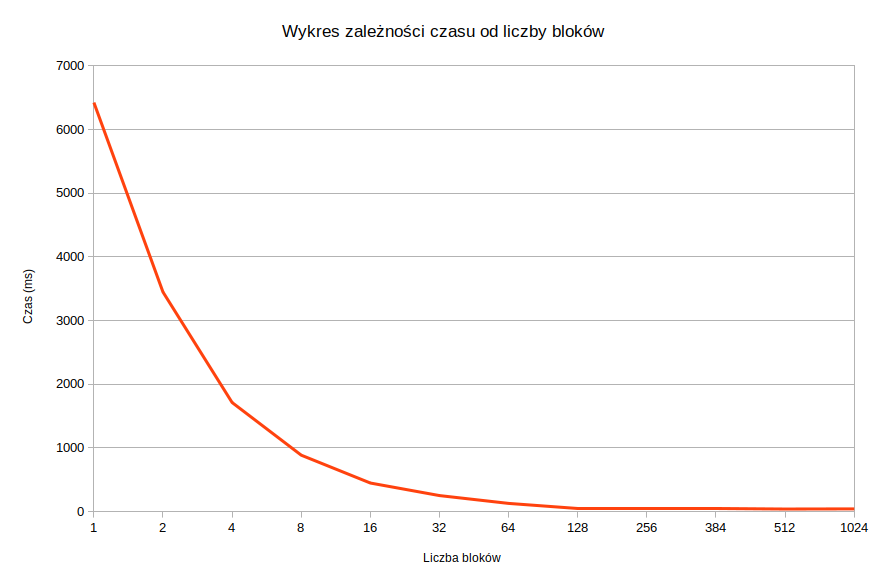
\includegraphics[width=0.9\textwidth]{WykresCzas.png}
  \caption{Wykres zależności czasu wykonywania obliczeń od liczby bloków}
\end{figure}


Jak można zauważyć, czas obliczeń znacząco się zmniejsza wraz z rozpoczęciem zwiększania liczby bloków. Wraz z wzrostem liczby bloków różnice pomiędzy sąsiednimi czasami stają się coraz mniejsze. Siatka została ustawiona na wartość 1 gdyż taka konfiguracja dawała najlepsze rezultaty. Liczba bloków na jakich program uzyskuje najlepsze rezultaty zależy od ilości liczb do przetestowania. W naszym przypadku dla zbioru testowego składającego się z 500 liczb, liczba bloków powyżej tej wartości nie dawała przyśpieszenia, gdyż każda liczba zostawała przypisana do jednego bloku. Dlatego też końcowy ilość bloków jest ustalana na podstawie ilości liczb zawartych w testowym pliku i jest ustalana podczas uruchomienia programu. Jest to rozwiązanie optymalne dla naszego algorytmu. W kernelu odbywa się podział liczb między bloki oraz wyznaczanie czy przesłana liczba jest liczbą pierwszą.

\end{document}
